\chapter{Analysis}
\label{chapter:ldmx:analysis}

One of the primary strengths of the \ac{ldmx} detector design is its ability to use the tagging and
recoil tracker system to reject a large number of background events by separating a nominal beam
with non-standard energy loss from a nominal beam with standard energy loss or even low-energy
beam. Moreover, the tagging and recoil tracker system gives \ac{ldmx} the potential to further
suppress backgrounds or potentially study \ac{dm} properties by studying the transverse momenta of
electrons recoiling from dark-bremsstrahlung candidate events.

While this design is optimal for a large number of \ac{eot}, the strategy has some limitations for
a low \ac{eot} data run. To limit multiple scattering which ruins momentum measurements, the
baseline detector configuration requires a thin ($\approx 0.1\mathrm{X}_0$) target. In the early
stages of \ac{ldmx}, when the total \ac{eot} will be lower, a different analysis strategy and
detector configuration may be optimal to probe the largest amount of the $y$--$m_\chi$ phase
space.\todo[introduce]{Provide MM search reach to help give conext to y and mchi.} The alternative
strategy would ignore the dedicated target inside the tracker volume and instead use the \ac{ecal}
as an active target. The \ac{eat} analysis channel for \ac{ldmx} thus has two primary purposes
which can be separated by the timeline over which they are relevant.
\begin{enumerate}
  \item \textbf{Short Term}: In early running, when the number of \ac{eot} is
        relatively small, the nominal \ac{mm} analysis will not have obtained
        significant reach into new \ac{dm} phase space (yet). The \ac{eat} channel
        serves here as a way to obtain world-leading sensitivity early in the lifetime
        of \ac{ldmx} and give the collaboration a first look at the data the apparatus
        has collected.
  \item \textbf{Long Term}: As \ac{ldmx} collects data, the \ac{mm}
        analysis enters into unexplored phase space and serves as a better discovery
        mechanism due to its access to the Tagger and Recoil trackers. The \ac{eat}
        channel, while struggling to suppress complicated backgrounds with relatively
        limited analysis handles, can operate ``orthogonally'' in the collected data
        since its primary selection (an approximately beam-energy electron passing
        through the Recoil tracker) is inverted relative to the \ac{mm} analysis
        (the electron passing through the Recoil tracker has significantly less
        energy than the beam).
\end{enumerate}

An initial study of the \ac{eat} analysis channel is the primary focus of \cref{part:ldmx} of this
thesis, focusing primarily on the first (short term) purpose. In this regard, we target an \ac{eot}
that is reasonable to accomplish early in the running of \ac{ldmx} and avoids particularly
intricate backgrounds. \num{1e13} \ac{eot} fits these requirements by avoiding the charged current
production of neutrinos and represents $\sim\qty{10}{percent}$ of the first full \ac{ldmx} dataset
obtainable within approximately a two weeks of beam time\footnote{ Assuming the \ac{ldmx} detector
  apparatus and beam delivery is operating according to specifications, we expect the beam to be
  delivered on a frequency of \qty{37.5}{\mega\hertz} with a duty cycle of $\approx$\num{0.5} and the
  number of electrons within each bunch to be Poisson distributed with $\mu=1$.
  $\qty{37.5}{\mega\hertz}\times0.5\times P(\mu=1,1) \times\qty{2}{week}\approx\num{1e13}$~\ac{eot}.
}. Since \ac{eat} is expected to be the \emph{first} physics analysis on \ac{ldmx} data, we want a
\emph{simple} and \emph{robust} analysis that can withstand the test of time and the complexities
of real data.

With these design goals in mind, a simple ``cut-and-count'' analysis has been developed. The
simplicity of this analysis is one of its strengths, enabling it to be applicable despite potential
surprises arising from first encounters with real data. The bulk of time and effort on this first
investigation was focused on making this investigation \emph{possible} via the introduction of
midshower process filtering and a dark bremsstrahlung simulatin process described in
\cref{chapter:ldmx:simulation}.

\section{Selection}
The core goal of most search analyses is to develop a selection that avoids events known to be
standard processes (i.e. backgrounds) while keeping events containing the process being searched
for (in this case, the production of \ac{dm} via dark-bremsstrahlung).
Both the \ac{eat} analysis channel and the primary \ac{mm} channel share the dark-bremsstrahlung
signature of missing energy within the \ac{ecal} relative to the known incident beam energy.
This allows for the first selection made to be shared between these two channels -- 
a requirement that the sum of the observed energy in the first twenty layers of the \ac{ecal}
is less than \qty{1.5}{\GeV} (\qty{3.16}{\GeV}) for a
\qty{4}{\GeV} (\qty{8}{\GeV}) beam.
This preliminary selection acts as the primary trigger for both of these analyses --
selecting events that resemble dark-bremsstrahlung via their lower-than-average
observed energy -- however, the \ac{eat} analysis channel in the early-running scenario
may not be collecting data with a fully calibrated energy scale at the trigger level.
The potential for mis-calibration motivates tightening this missing energy requirement
by \qty{400}{\mega\electronvolt} as well as requiring the sum to be performed over all thirty-four
layers of the \ac{ecal} instead of only the first twenty.

\begin{figure}[htb]
    \centering
    \begin{tabular}{cc}
         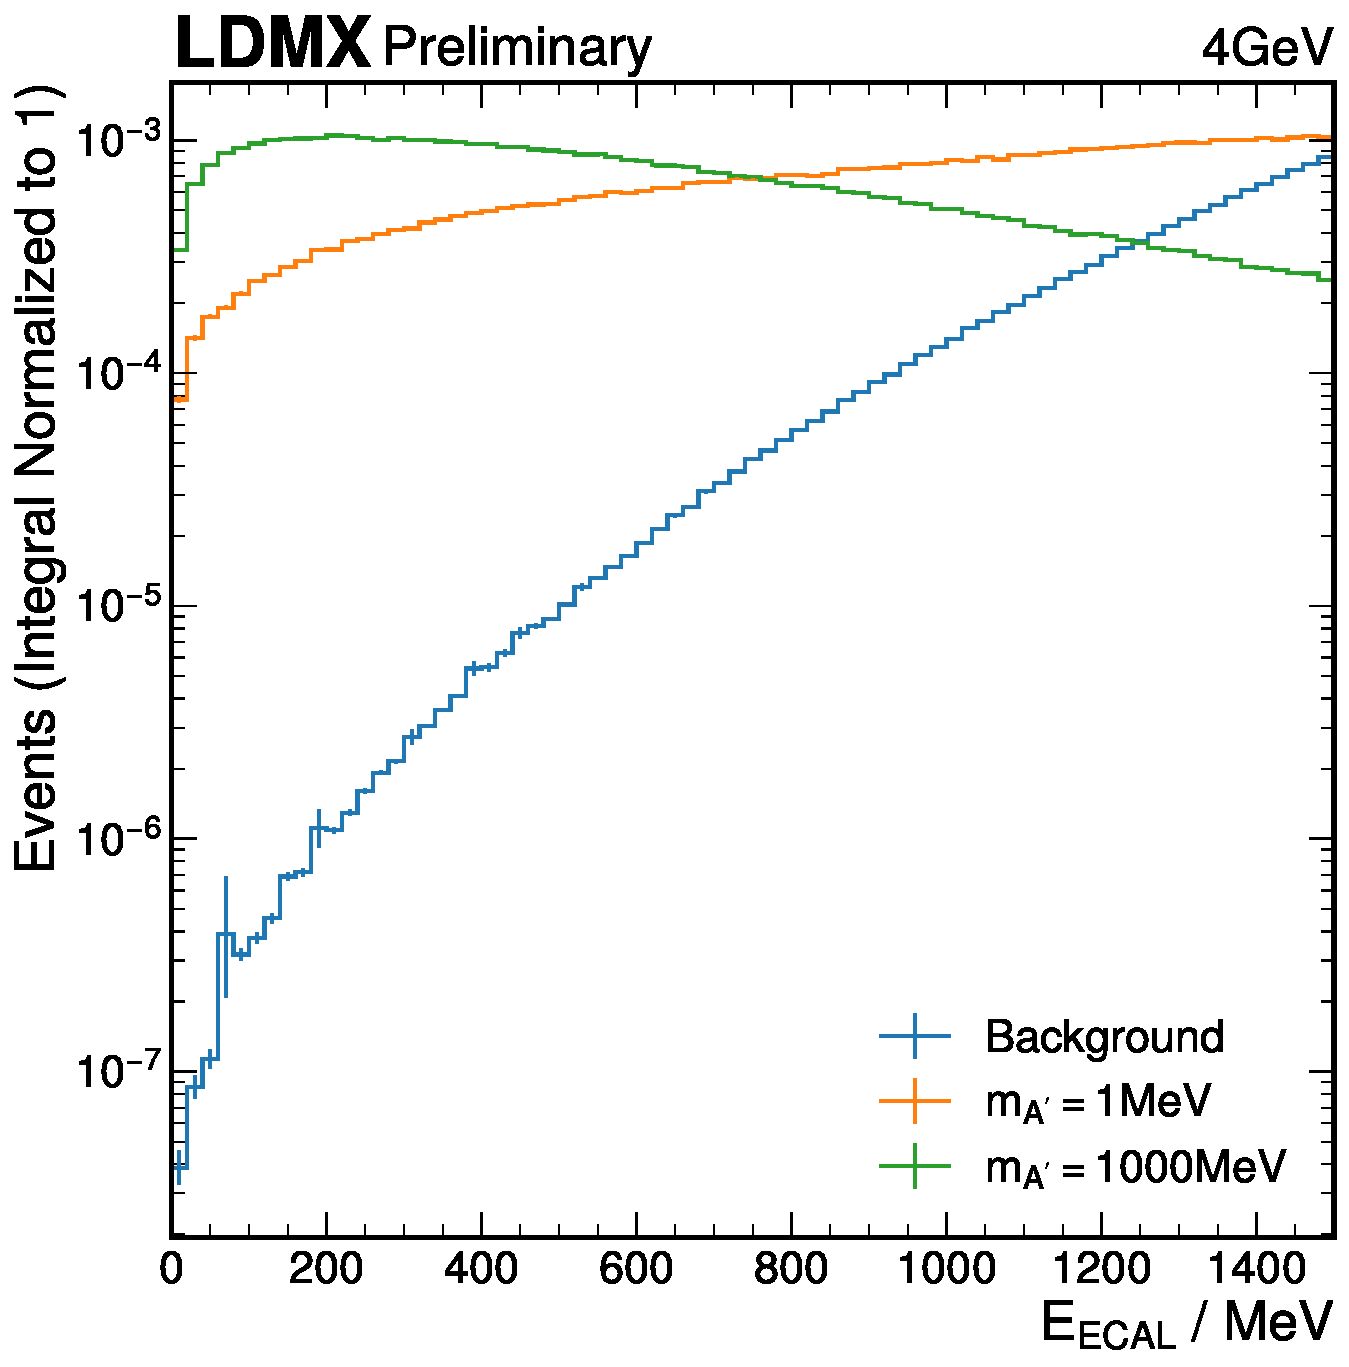
\includegraphics[width=0.48\textwidth]{figures/ldmx/analysis/energy-after-trigger-4gev.pdf}
         &
         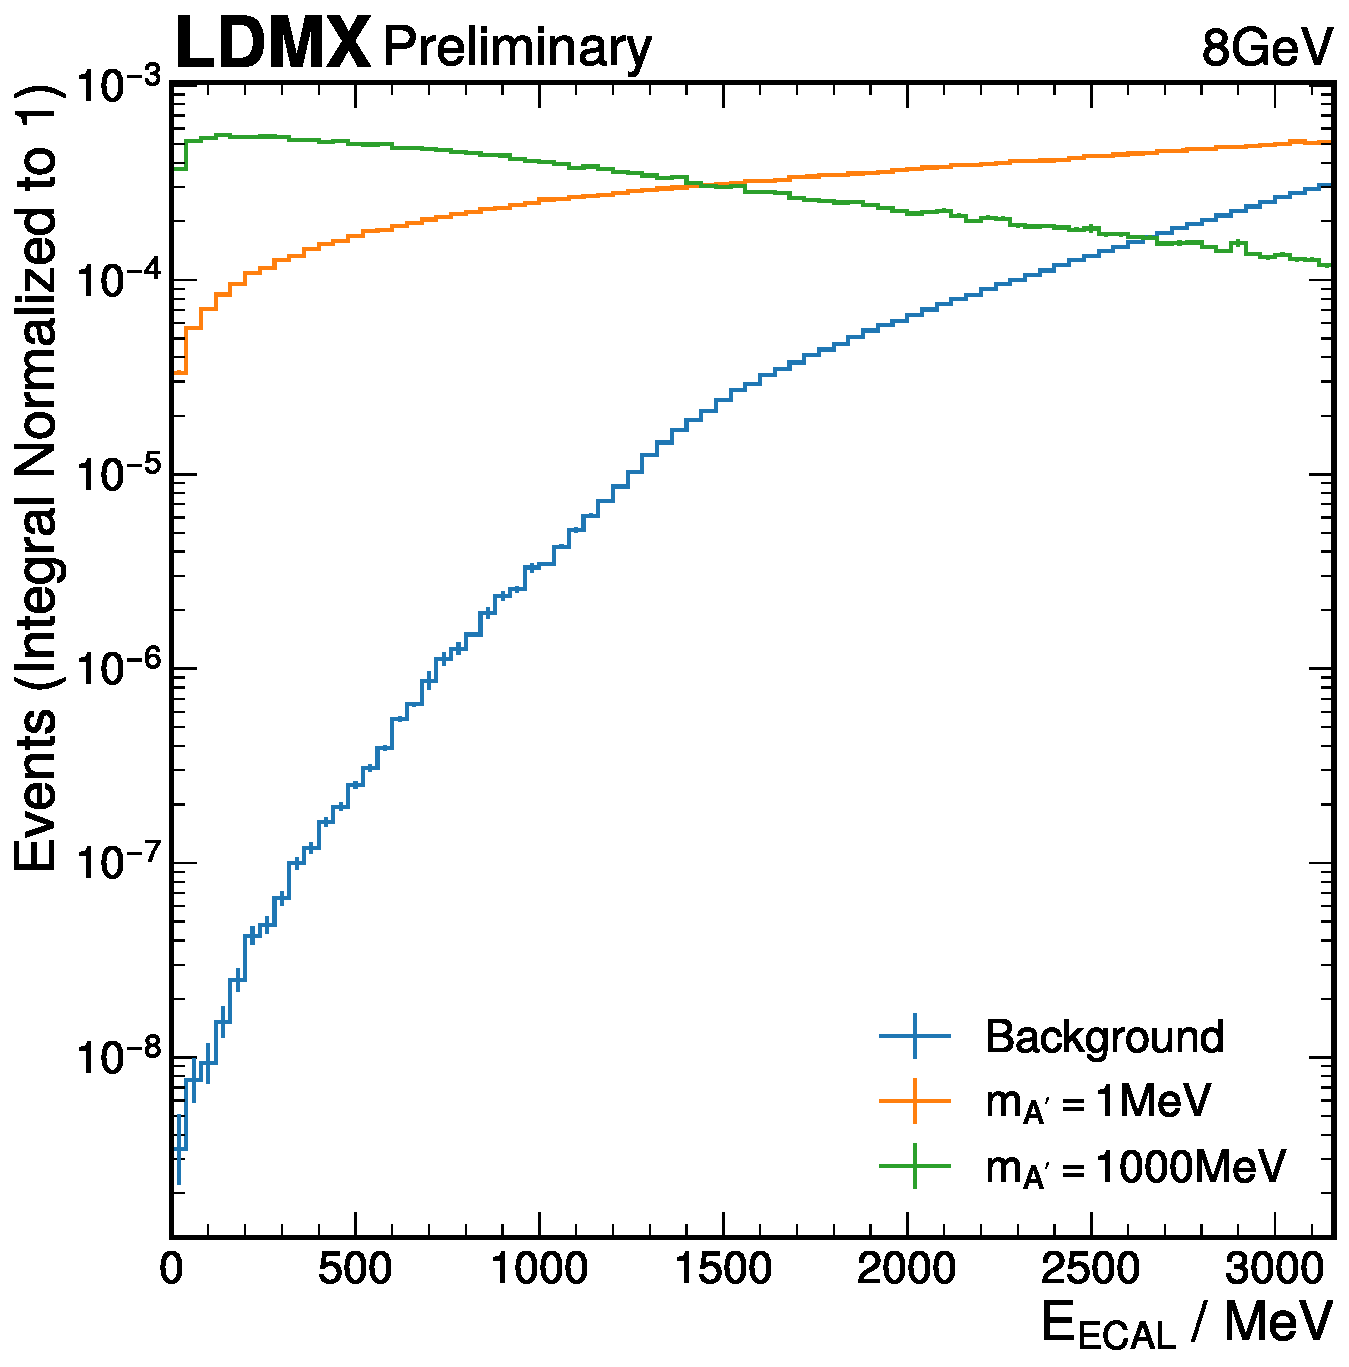
\includegraphics[width=0.48\textwidth]{figures/ldmx/analysis/energy-after-trigger-8gev.pdf}
    \end{tabular}
    \caption{
    The total reconstructed energy in all layers of the ECal ($E_\text{ECAL}$) as a fraction of the beam energy
    $E_\text{Beam}$ for all samples that pass the trigger threshold.
    The signal and background distributions are normalized such that their integral is one.
    The \qty{4}{\GeV} beam is shown on the left and the \qty{8}{\GeV} beam is shown
    on the right.
    The events falling into bins with $E_\text{ECAL} > \qty{1.5}{\GeV}~(\qty{3.16}{\GeV})$
    for \qty{4}{\GeV} (\qty{8}{GeV}) are omitted from this plot but included in efficiency calculations.
    }
    \label{fig:ecal_rec_energy}
\end{figure}

\section{Cut and Count}
List cuts for different beams, provide final background yields and signal efficiencies.

\section{Systematics and Background Uncertainty}
Calibration errors (i.e. putting requirements on the accuracy of initial calibration for this
analysis to function) Estimate of background uncertainty informing how the toy counting experiments
are done when estimating reach.

\section{Reach}
Display reach of ME analysis with different background hypotheses and signal efficiencies motivated
by findings above.

